%!TEX root = Manuscript.tex

\chapter{Introduction}
\label{chap:intro}
\minitoc

\section{Motivation and objectives}
\subsection{Why are historical images interesting}
Historical (i.e., analogue or archival) aerial images play an important role in providing unique information about evolution of land-covers. 
They are valuable assets for a wide range of applications such as (1) analyzing of natural disasters (e.g., earthquake, landslide, volcano, flood, avalanche, etc), (2) eco-environmental monitoring (e.g., forest, atmosphere, glacier, water, coastline, etc), (3) urban expansion and (4) environmental pollution and protection and so on.
\par
Historical aerial images have been regularly acquired since the 1920’s by mapping, military or cadastral agencies all over the world. A mass amount of them have been digitized and made accessible through web services~\cite{sebastien2019archiving,earthexplorer,remonterletemps}. 
For example, according to a survey taken place at the beginning of 2017 in Europe~\cite{sebastien2019archiving}, there are approximately 50 million of aerial images archived in Europe, with around 37.8\% of them digitized. 
The images are of high spatial resolution, and are acquired in stereoscopic configuration, allowing for 3D restitution of territories. 
They are often accompanied by metadata, in most cases including the camera focal length, flight height, scale and the physical sensor size, which are usually saved or mentioned on the films. Other metadata such as flight plans, camera calibration certificates or orientations are not commonly available. 
\par
When the camera calibration parameters are unknown, they should be evaluated by a procedure called self-calibrating bundle adjustment. \ac{GCP}s are required, otherwise inaccurately estimated camera parameters will lead to systematic error surfaces called dome effect (i.e., bowl effect).
Generally, \ac{GCP}s originate from (1) field surveys \cite{micheletti2015application,walstra2004time,cardenal2006use}, (2) recent orthophotos and \ac{DSM} \cite{nurminen2015automation,ellis2006measuring,fox2008unlocking} and (3) recent satellite images \cite{ellis2006measuring,ford2013shoreline}. The most challenging part is to identify the \ac{GCP}s on the historical images, which is not easy due to inevitable scene changes. \ac{GCP}s are usually manually measured with the help of recent photos, however, it is still monotonous and time-consuming. 
There is an urgent need to automatically identify corresponding points (i.e., matches) on historical and recent images.\\
When users are only interested in comparing different historical epochs, the self-calibration can be accomplished without \ac{GCP}s. Matches between different epochs would serve as observations in bundle adjustment to eliminate the systematic errors in surfaces. In conclusion, the bottleneck of historical image self-calibration is recovering matches on images taken at different times (i.e., multi-epoch).

\subsection{How to match multi-epoch historical images}
However, matching multi-epoch historical images remains challenging, despite the fact that there exists a large number of image matching algorithms with their effectiveness proven on modern images. The reasons include:
\begin{enumerate}
	\item Multi-epoch images are often acquired at different times of day and in various weathers and seasons, which unavoidably leading to appearance differences.
	\item The scene changes over time due to anthropogenic phenomena (e.g., urban planning) or natural ones (e.g., earthquake), especially for large time gaps.
	\item Multi-epoch images often exhibit heterogeneous spatial resolutions, accompanied with different acquisition conditions (sensors, spectral channels, etc).
	\item Historical images are often facing low radiometric quality, including low contrast, image noise, deterioration due to the aging of films, or even scratches on the films.
\end{enumerate}
Simply applying \textit{state-of-the-art} feature matching methods (e.g., SIFT~\cite{lowe2004distinctive} or SuperGlue~\cite{sarlin2020superglue}) on multi-epoch image pair often leads to unsatisfactory results. An example is given in Figure~\ref{MultiEpochImgPair}. A pair of multi-epoch images are demonstrated with red rectangles indicating the overlapping area in Figure~\ref{MultiEpochImgPair}(a). The left and right images are taken at the same place in 1954 and 1970 individually. The scene changed significantly, a lot of new buildings arose, the color tones were very different. In Figure~\ref{MultiEpochImgPair}(b-d), the matching result of SIFT, SuperGlue and Ours are displayed for comparison. As can be seen, SIFT failed to find any matches. SuperGlue recovered 369 matches, most of which seem good, but at a closer look the details reveal poor localization precision. Our method found 1463 matches with high accuracy, thanks to the help of (1) 3D geometry and (2) the divide and conquer (i.e., rough-to-precise) strategy, which are elaborated in the following texts.
\begin{figure*}[htbp]
	\begin{center}
		\subfigure[Multi-epoch image pair]{
			\begin{minipage}[t]{0.45\linewidth}
				\centering
				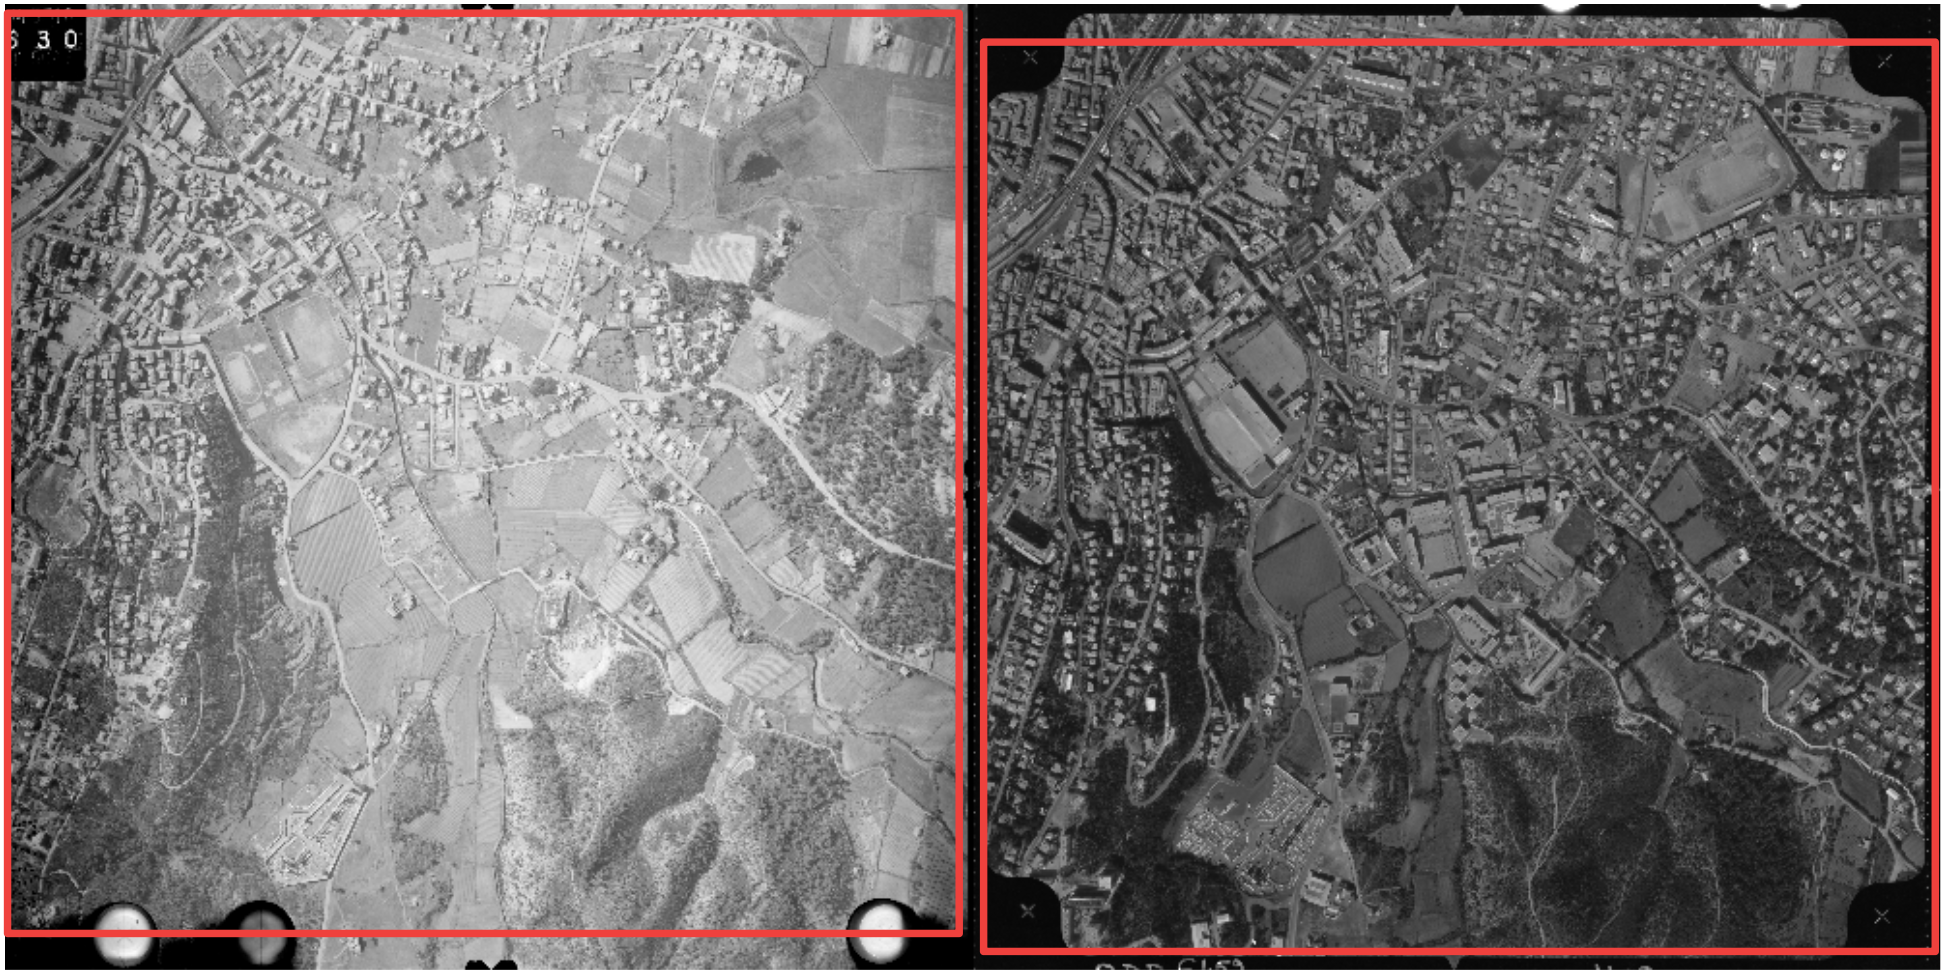
\includegraphics[width=6.2cm]{images/Chapitre1/OIS-Reech_IGNF_PVA_1-0__1954-03-06__C3544-0211_1954_CDP866_0630_OIS-Reech_IGNF_PVA_1-0__1970__C3544-0221_1970_CDP6452_1409.png}
			\end{minipage}%
		}
		\subfigure[Result of SIFT (0 matches)]{
	\begin{minipage}[t]{0.45\linewidth}
		\centering
		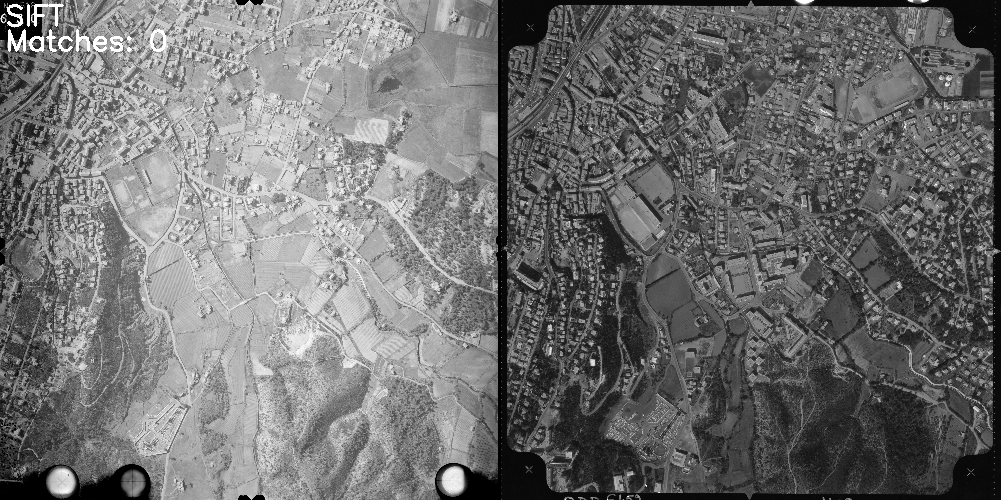
\includegraphics[width=6.2cm]{images/Chapitre1/Homol-SIFT_OIS-Reech_IGNF_PVA_1-0__1954-03-06__C3544-0211_1954_CDP866_0630_OIS-Reech_IGNF_PVA_1-0__1970__C3544-0221_1970_CDP6452_1409.png}
	\end{minipage}%
}
		\subfigure[Result of SuperGlue]{
	\begin{minipage}[t]{0.45\linewidth}
		\centering
		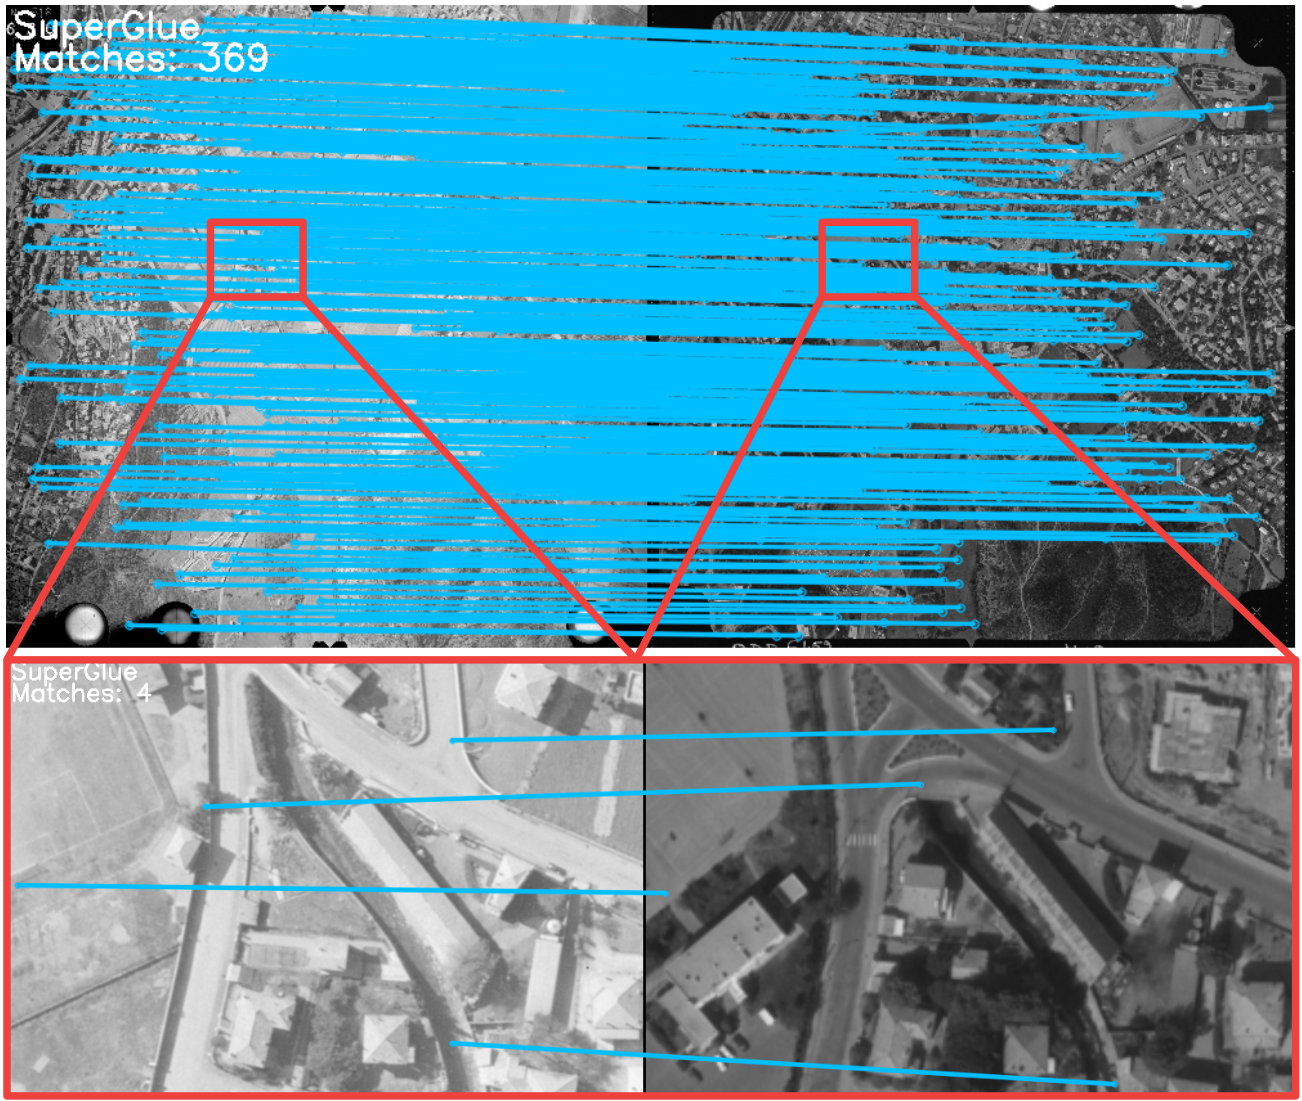
\includegraphics[width=6.2cm]{images/Chapitre1/Homol-SuperGlue_OIS-Reech_IGNF_PVA_1-0__1954-03-06__C3544-0211_1954_CDP866_0630_OIS-Reech_IGNF_PVA_1-0__1970__C3544-0221_1970_CDP6452_1409.png}
	\end{minipage}%
}
		\subfigure[Result of Ours]{
	\begin{minipage}[t]{0.45\linewidth}
		\centering
		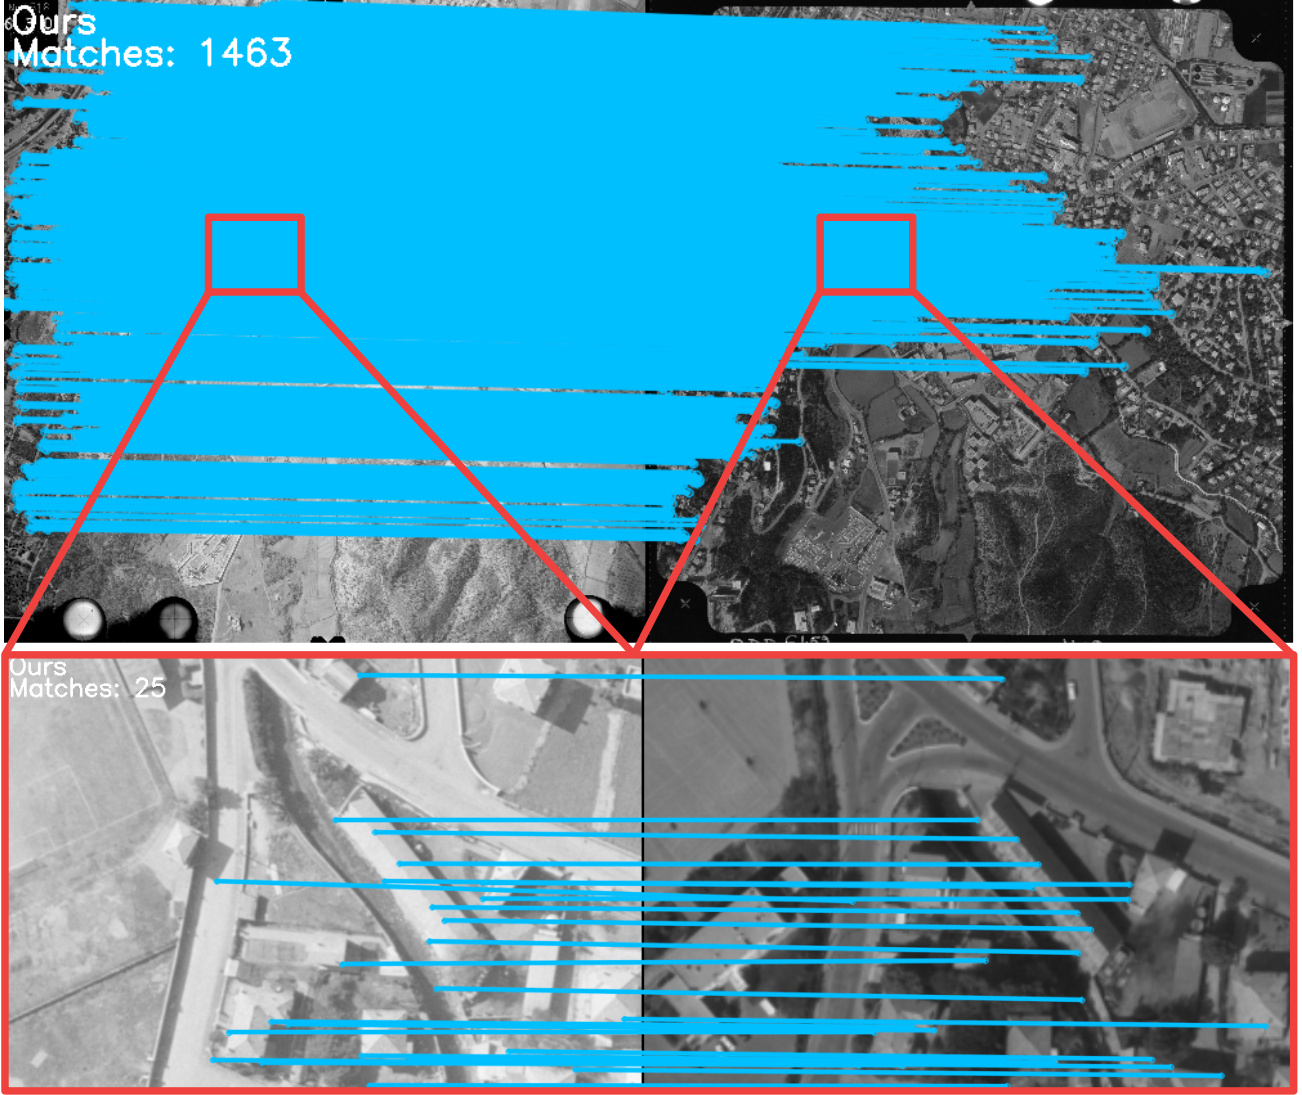
\includegraphics[width=6.2cm]{images/Chapitre1/Homol-Ours_OIS-Reech_IGNF_PVA_1-0__1954-03-06__C3544-0211_1954_CDP866_0630_OIS-Reech_IGNF_PVA_1-0__1970__C3544-0221_1970_CDP6452_1409.png}
	\end{minipage}%
}
		\caption{(a) A pair of multi-epoch images with red rectangles indicating the overlapping area. (b-d) Matching result of SIFT, SuperGlue and Ours.}
		\label{MultiEpochImgPair}
	\end{center}
\end{figure*}

%\subsubsection{Take advantage of 3D geometry}
\paragraph{Advantages of 3D geometry}
RGB images are widely used for image matching. However, they have the following shortcomings:\\
(1) Their appearances change over time (see Figure~\ref{AppearanceChange}), and over varying view angles on non-Lambertian surfaces (see Figure~\ref{PoorlyTextured}).\\
(2) Self similarities (e.g., repetitive patterns) favor false matches (see Figure~\ref{PoorlyTextured}).\\
Fortunately, 3D geometry such as \ac{DSM} makes up for these shortcomings perfectly. As can be seen in Figure~\ref{AppearanceChange}, the RGB images look very different because the scene changed a lot. However, the corresponding \ac{DSM}s look similar, which is reasonable, as the 3D landscape is more stable over time. Besides, \ac{DSM} is more distinctive than RGB image when it comes to non-Lambertian surfaces and repetitive patterns, as shown in Figure~\ref{PoorlyTextured}. 
Even though 3D geometry lacks textures and details compared to RGB image, it serves as an ideal supplement. Besides, it plays an important role in providing the 3D information for establishing 3D Helmert transformation model between epochs to (1) move different epochs into the same coordinate frame and (2) remove false matches in a RANSAC routine which is more reliable than 2D transformation models.

\begin{figure*}[htbp]
	\begin{center}
		\subfigure[RGB image 1971]{
			\begin{minipage}[t]{0.45\linewidth}
				\centering
				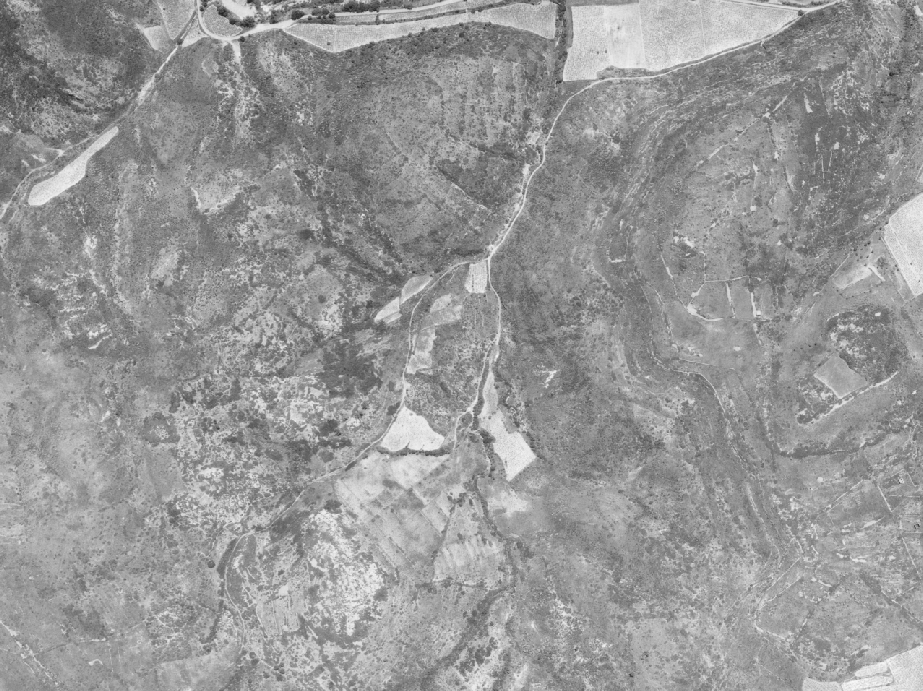
\includegraphics[width=6.2cm]{images/Chapitre1/AppearanceChangeRGBL.png}
			\end{minipage}%
		}
		\subfigure[RGB image 2015]{
			\begin{minipage}[t]{0.45\linewidth}
				\centering
				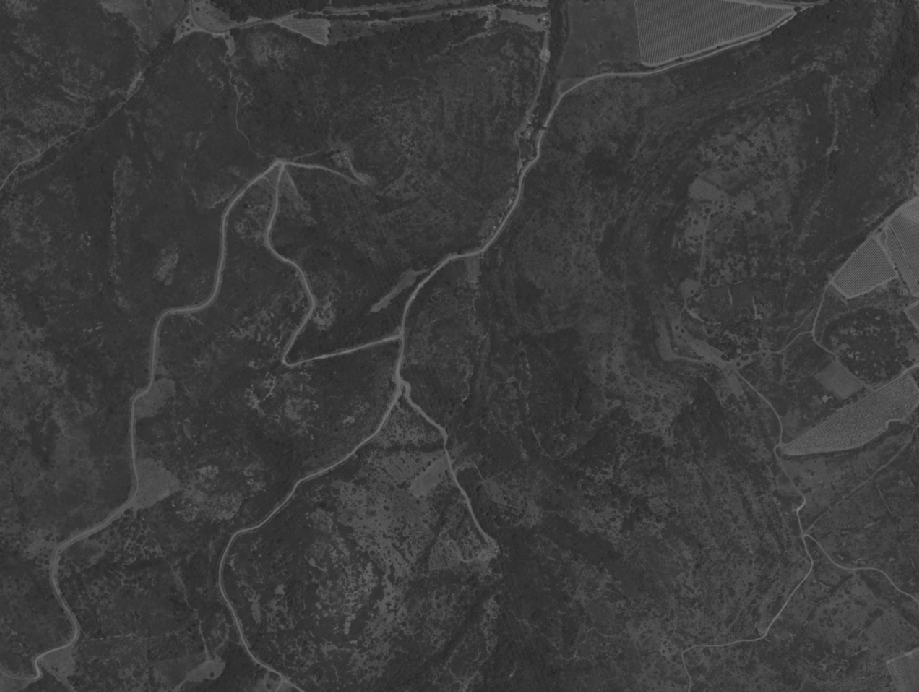
\includegraphics[width=6.2cm]{images/Chapitre1/AppearanceChangeRGBR.png}
			\end{minipage}%
		}
		\subfigure[\ac{DSM} 1971]{
			\begin{minipage}[t]{0.45\linewidth}
				\centering
				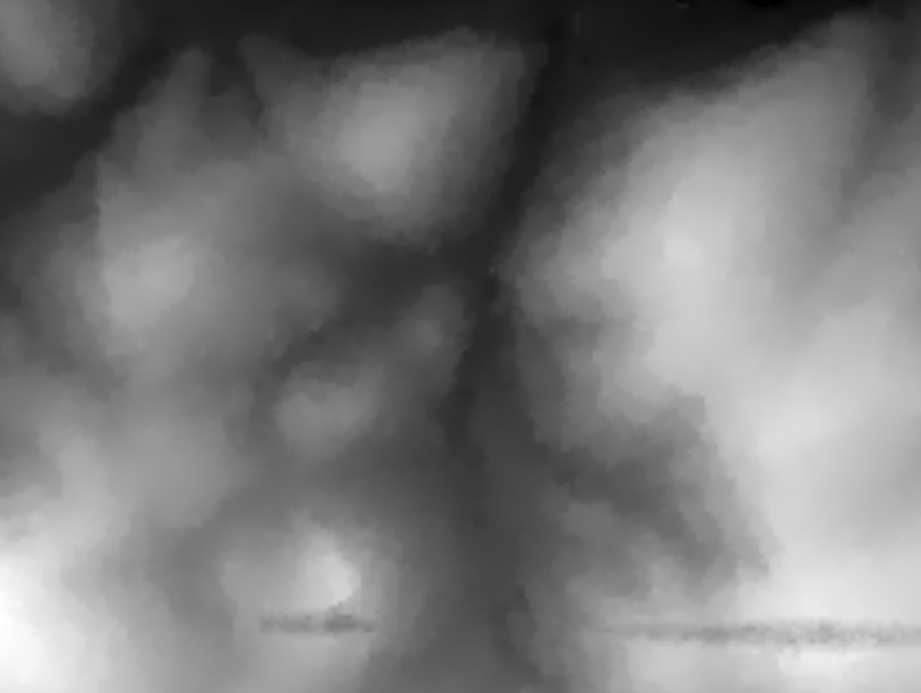
\includegraphics[width=6.2cm]{images/Chapitre1/AppearanceChangeDSML.png}
			\end{minipage}%
		}
		\subfigure[\ac{DSM} 2015]{
			\begin{minipage}[t]{0.45\linewidth}
				\centering
				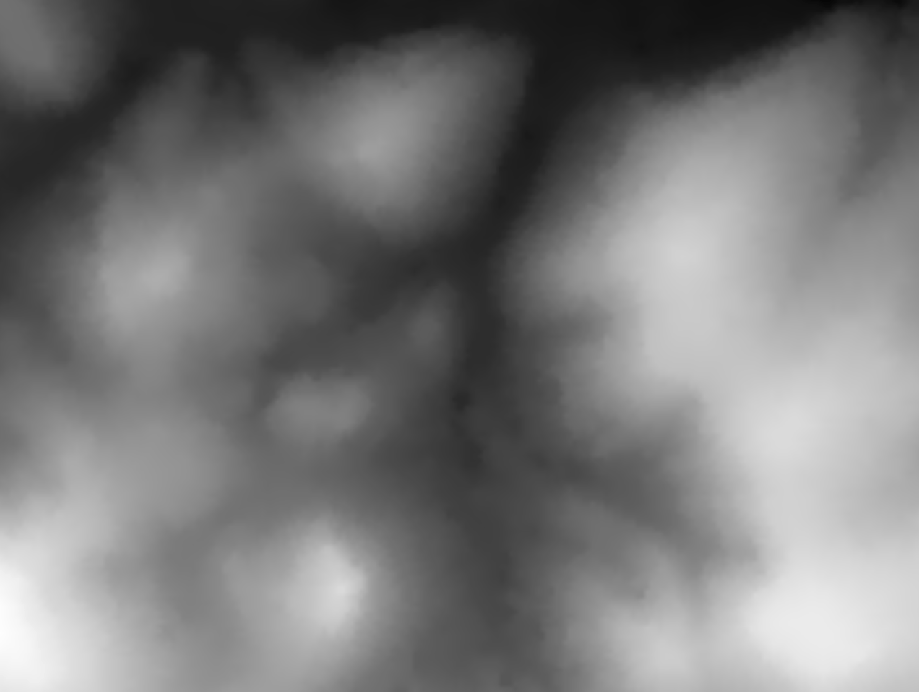
\includegraphics[width=6.2cm]{images/Chapitre1/AppearanceChangeDSMR.png}
			\end{minipage}%
		}
		\caption{The same zone observed in different times. The RGB images changed a lot while the \ac{DSM}s stayed stable over time.}
		\label{AppearanceChange}
	\end{center}
\end{figure*} 


\begin{figure*}[htbp]
	\begin{center}
		\subfigure[RGB image 1971]{
			\begin{minipage}[t]{0.45\linewidth}
				\centering
				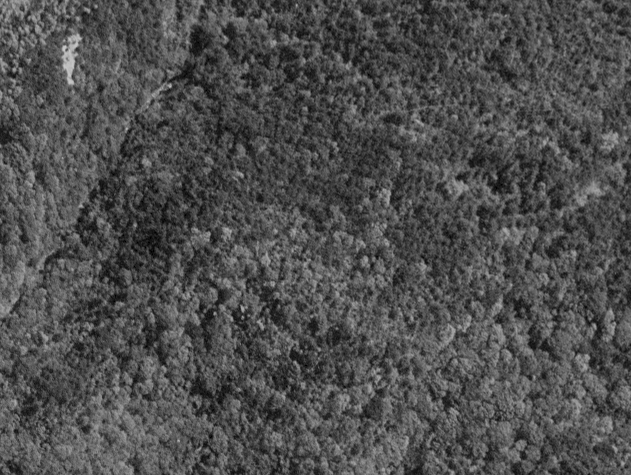
\includegraphics[width=6.2cm]{images/Chapitre1/PoorlyTexturedRGBL.png}
			\end{minipage}%
		}
		\subfigure[RGB image 2015]{
			\begin{minipage}[t]{0.45\linewidth}
				\centering
				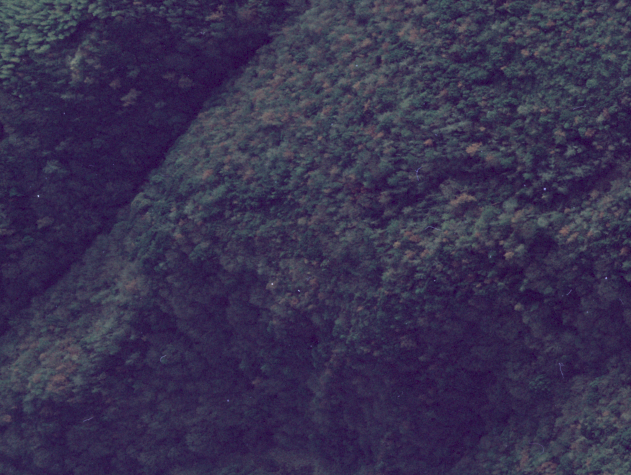
\includegraphics[width=6.2cm]{images/Chapitre1/PoorlyTexturedRGBR.png}
			\end{minipage}%
		}
		\subfigure[\ac{DSM} 1971]{
			\begin{minipage}[t]{0.45\linewidth}
				\centering
				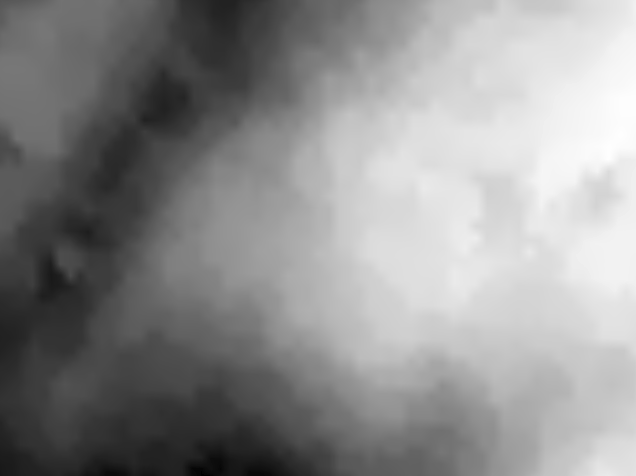
\includegraphics[width=6.2cm]{images/Chapitre1/PoorlyTexturedDSML.png}
			\end{minipage}%
		}
		\subfigure[\ac{DSM} 2015]{
			\begin{minipage}[t]{0.45\linewidth}
				\centering
				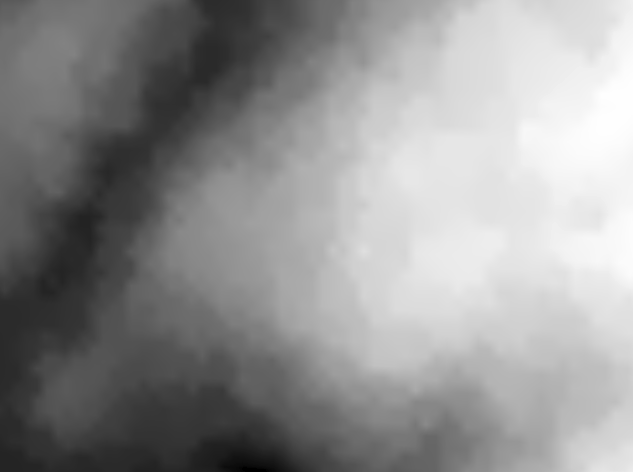
\includegraphics[width=6.2cm]{images/Chapitre1/PoorlyTexturedDSMR.png}
			\end{minipage}%
		}
		\caption{The same vegetation observed in different times. Non-Lambertian reflection and self similarities present in RGB images, while the \ac{DSM}s stay distinctive.}
		\label{PoorlyTextured}
	\end{center}
\end{figure*} 

%\subsubsection{Rough-to-precise strategy}
\paragraph{Divide and Conquer}
Since the task of recovering robust and precise matches on multi-epoch image pairs is difficult, we divide the task into two sub-tasks and conquer them individually with the rough-to-precise strategy. It is illustrated in Figure~\ref{rough-to-precise}. The two sub-tasks includes:\\
\begin{enumerate}
	\item Rough co-registration, as illustrated in Figure~\ref{rough-to-precise}(b). Its goal is to roughly align the multi-epoch image pairs by focusing on robustness and relaxing the requirement for accuracy.
	\item Precise matching, as illustrated in Figure~\ref{rough-to-precise}(c). It refines the matches predicted by the rough co-registration result by searching only the local neighborhood to reduce ambiguity.
\end{enumerate}

\begin{figure*}[htbp]
	\begin{center}
		\subfigure[Example of an inter-epoch image pair]{
			\begin{minipage}[t]{1\linewidth}
				\centering
				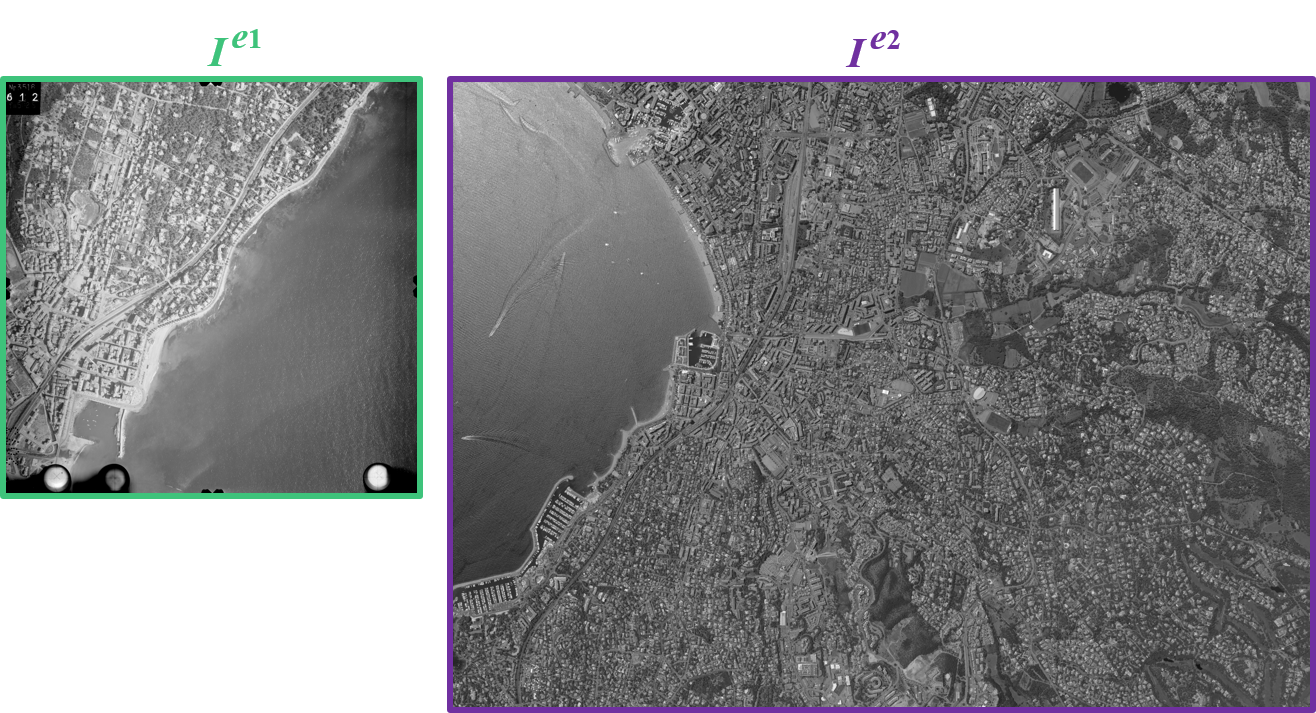
\includegraphics[width=1\columnwidth]{images/Chapitre1/imagepair.png}
			\end{minipage}%
		}
		\subfigure[Rough co-registration]{
			\begin{minipage}[t]{1\linewidth}
				\centering
				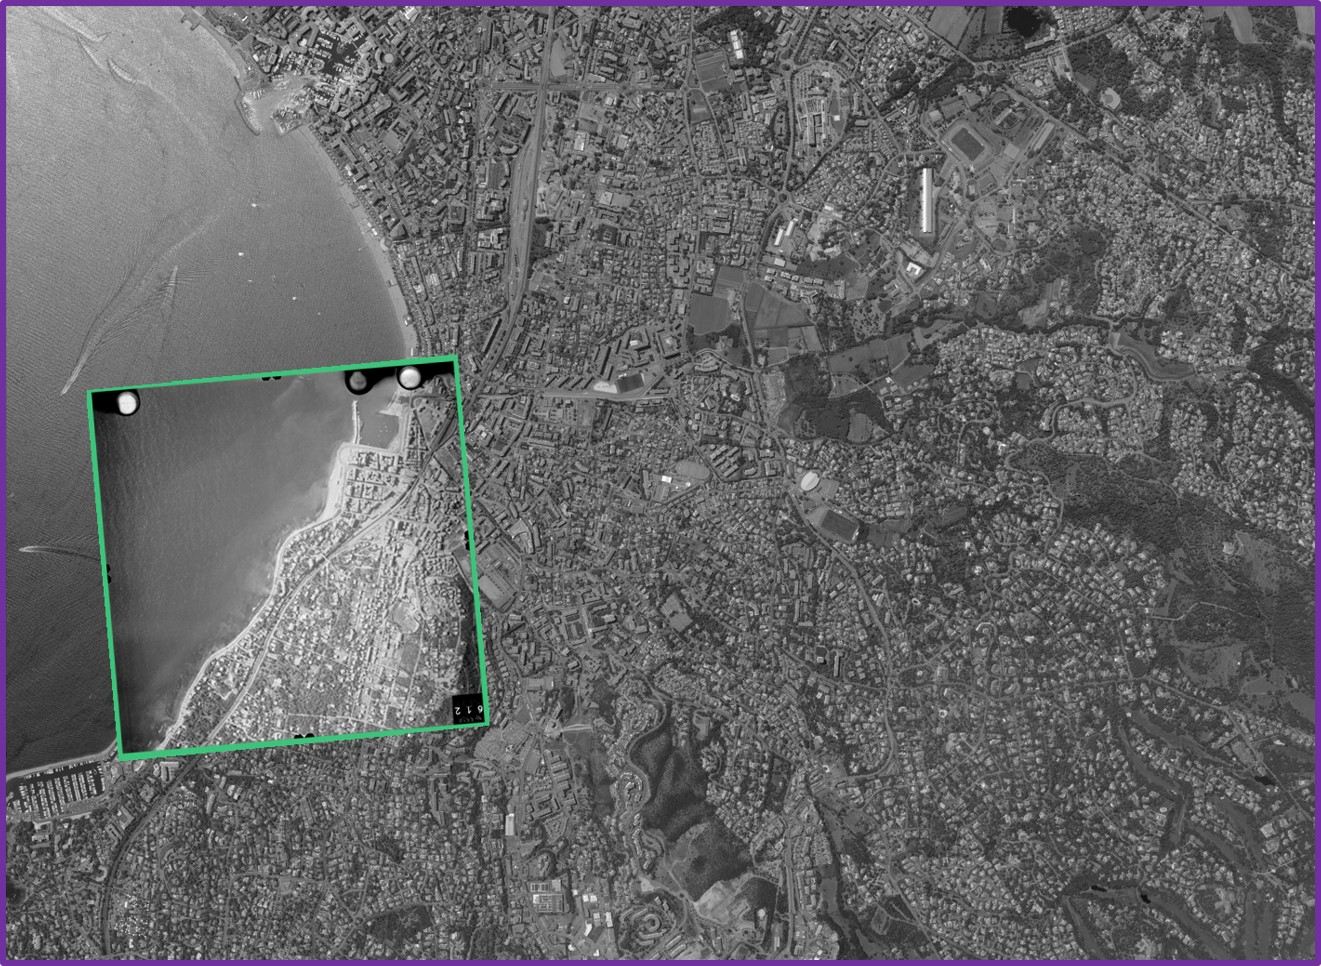
\includegraphics[width=0.68\columnwidth]{images/Chapitre1/CoReg.jpg}
			\end{minipage}%
		}
		\subfigure[Precise matching]{
			\begin{minipage}[t]{1\linewidth}
				\centering
				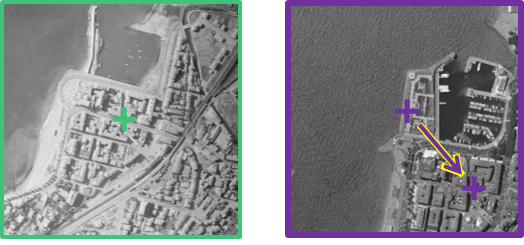
\includegraphics[width=0.55\columnwidth]{images/Chapitre1/Precise.png}
			\end{minipage}%
		}
		\caption{ Rough-to-precise strategy. (a) An example of an inter-epoch image pair to be matched. $I^{e_1}$ and $I^{e_2}$ represents images take at $epoch_1$ and $epoch_2$ individually. (b) Illustration of rough co-registration between $I^{e_1}$ and $I^{e_2}$. As a result, $I^{e_1}$ is roughly aligned with $I^{e_2}$. (c) Illustration of precise matching. For keypoints in $I^{e_1}$ (green cross), a location is predicted in $I^{e_2}$ (purple cross) based on rough co-registration, whose local neighborhood will be searched to find the precise match (yellow cross).}
		\label{rough-to-precise}
	\end{center}
\end{figure*}

\section{Contributions}
\label{sec:contributions}
In this thesis we present rough-to-precise pipelines for matching multi-epoch images. They are suitable for aerial, satellite and mixed images, which open the possibility of geo-referencing millions of historical images without requiring any \ac{GCP}s. 
Six variants are provided for the rough co-registration stage and two variants for the precise matching stage. Each variant has its own characteristic:\\
\begin{enumerate}
	\item For rough co-registration variants: (1) the ones based on the idea of matching \ac{DSM}s generally lead to the most robust results; (2) the ones that match orthophotos could serve as an alternates in rare scenarios of perfectly flat terrain where \ac{DSM}s fail to provide useful information; (3) the others that match original image pairs often lead to less satisfactory results, but they are the only options suitable for terrestrial images.
	\item For precise matching variants: (1) $Patch$ is based on learned matching methods, it generally results in more matches as it is more invariant over time. (2) $Guided$ is based on hand-crafted methods, it is more efficient in terms of the use of memory and CPU resources as it doesn't involve resampling patches, which is necessary for $Patch$. 
\end{enumerate}
\par
Our pipelines aim to unlock the potential of historical images for tracking environmental conditions. 
We are currently collaborating with several institutes to apply our pipelines in different applications, including:
\begin{enumerate}
	\item Institut de Physique du Globe de Paris (IPGP) and Korea Institute of Geoscience and Mineral Resources (KIGAM) for analyzing deformations of the earth crust to understand the seismic events.
	\item National Research Council, Research Institute for Hydrogeological Protection (CNR-IRPI) for analyzing landslide evolution in Italy.
	\item Department of Earth and Environmental Sciences in University of Pavia for analyzing badland evolution in Europe.
\end{enumerate}
\par
We also developed two thorough tutorials accompanied with test datasets to familiarize users with our pipelines implemented in MicMac\cite{HistoPcode} (more details are introduced in Appendix \ref{chap:appendixC}):
\begin{enumerate}
	\item Tutorial of matching aerial images \cite{tuto-aerial} 
	\item Tutorial of matching mixed images (i.e., aerial and satellite images) \cite{tuto-mixed} 
\end{enumerate}

\par
Publications of the author:
\begin{enumerate}
	\item Lulin Zhang, Ewelina Rupnik and Marc Pierrot-Deseilligny. Feature matching for multi-epoch historical aerial images. ISPRS Journal of Photogrammetry and Remote Sensing, 182, 176-189, 2021.
	\item Lulin Zhang, Ewelina Rupnik and Marc Pierrot-Deseilligny.	Guided feature matching for multi-epoch historical image blocks pose estimation. In ISPRS Ann. Photogramm. Remote Sens. Spatial Inf. Sci., 2020.
\end{enumerate}
We also provide video \cite{HistoPVideo}, slides \cite{HistoPSlides} and project website \cite{HistoPProj} to improve the visibility of our work.

\section{Organization of the thesis}
This thesis presents fully automatic pipelines to match multi-epoch images.
A brief presentation of the \textit{state-of-the-art} is given in \textbf{Chapter}~\ref{chap:review}. \\

In \textbf{Chapter}~\ref{chap:ApplicationsAndDatasets}, applications as well as 5 sets of representative datasets are introduced, which are latter used to test our pipelines.\\

In \textbf{Chapter}~\ref{chap:RoughCoReg}, six rough co-registration variants are elaborated to roughly align the whole block by building a globally consistent transformation model between different epochs.\\

In \textbf{Chapter}~\ref{chap:Precisematching}, two precise matching variants are introduced to get accurate matches under the guidance of roughly co-registered orientations and \ac{DSM}s.\\

Finally, in \textbf{Chapter} ~\ref{chap:conclusion} conclusion and perspective are given.\\

